\chapter{Datasets}
Now we consider the study case of the datasets:
\begin{itemize}
	\item  N body problem
	\item Two body problem
	\item Threebody problem
	\item N pendelum
\end{itemize}
First we will mathematically describe the system and later we will explain how to prepare and create trajectories corresponding to their starting point/initial value. 


\section{Oscilator}
As we already shown the oscillator solution, we could show solution of the oscilator trough hamiltonian equations.
For this we will use Kinetic Energy $T =\frac{1}{2}mv^2$ and Potentional energy $U = \frac{1}{2}kx^2$. Using the momentum $p = mv$ we can rewrite our 
Kinetic energy as  $T =\frac{1}{2m}p^2$.\\
Using Hamiltonian Energy definition we obtain following equation: 
\begin{equation}
	\mathcal{H} = \frac{1}{2m}p^2 + \frac{1}{2}kx^2
\end{equation} 
This case is trivial.
We could get $\dot{x}$ and $\dot{p}$ trough hamiltonian equations $\dot{q} = \frac{\partial H}{\partial p}$ and $\dot{p} = - \frac{\partial H}{\partial q}$,
or we could compare Hamiltonian with elipse formula
\begin{equation}
	1 = \frac{x^2}{a^2} + \frac{y^2}{b^2},
\end{equation} and set the components in parametric equation\begin{equation}
(x,y) = (a\cos(\phi),b\sin(\phi)) \rightarrow(p,q) = \left(\sqrt{2Hm}\cos(\phi),\sqrt{\frac{2H}{k}}\sin(\phi)\right)
\end{equation} of the ellipse.\\ This equation represents kinematics of the oscilator. To find periodicity let say that $\phi = \omega t + \Phi $ and we know that the $p = mx$, with this equation we can calculate $\omega$.
\begin{eqnarray}
	p &=& m\dot{x} =\sqrt{2Hm}\cos(\omega t + \Phi), \\
	\dot{x} &=& \sqrt{\frac{2H}{m}}\cos(\omega t + \Phi),\\
		x &=& \int \sqrt{\frac{2H}{m}}\cos(\omega t + \Phi)dt = \frac{1}{\omega}\sqrt{\frac{2H}{m}}\sin(\omega t + \Phi) = \sqrt{\frac{2H}{k}} \sin(\omega t + \Phi),\\
	\omega &=& \sqrt{\frac{k}{m}} 
\end{eqnarray}  




The oscliator has harmonic, periodic movement which means that after some time $T$ the movement will be repeated $x(t_0) = x(t_N)$. With that property we can calculate the period over circle circumference:
\begin{equation}
	T = \frac{2\pi}{\omega}
\end{equation}

With this we can create a dataset within the program code. For coding we used framework $\texttt{pytorch}$ to calculate this dataset numerically.\\
For the obtain the solution of ODE we used package \texttt{torchdiffeq}\cite{torchdiffeq} to solve numerical equation with dopri5 method, which is most accurate method for solving ODEs.\\
To create unique trajectories for the dataset we just need to specify energy region.


\section{N-body problem}
N-body problem is most complex problem in physics. It describes a movement of bodies in the free space. There are no conditions and there are multitude of solutions. This problem is even a topic in quantum theory.\\ We will just observe an compute real or deterministic trajectories of this problem.\\ 
In Newtonian formulation the N-body problem is
\begin{equation}
m_i\ddot{\mathbf{x}}_i = -\sum_{i\neq j, j=1}^nG\frac{m_im_j(\mathbf{x}_i-\mathbf{x}_j)}{||\mathbf{x}_i-\mathbf{x}_j||^3}
\end{equation} 
and its Hamiltonian:
\begin{equation}
	\mathcal{H} =\sum_i^n \frac{1}{2m_i}||\mathbf{p}_i||^2 - \sum_{1<i,j<n,i\neq j}\frac{Gm_im_j}{||\mathbf{x}_i-\mathbf{x}_j||}
\end{equation} 
for $i \in[1,n].$
N body problem is very complex problem because we need to achieve a conservative property of the Hamiltonian in the system.\\
The biggest issue in this dataset are the crashes between the bodies.
This can be resolved with simple trick adding the $\epsilon$ to fix maximal potential energy
\begin{equation}
	- \sum_{1<i,j<n,i\neq j}\frac{Gm_im_j}{||\mathbf{x}_i-\mathbf{x}_j||+\epsilon}.
\end{equation}
We secured that the value in the dominator never reaches 0. This is important because we use numerical solvers to create trajectories. If we have energy which achieves very big difference in values between two time steps, our solution will be inaccurate.  For calculation of such trajectories we are forced not to calculate over the Hamiltonian equations, but to calculate the trajectories using acceleration, velocity and position of the bodies trough some symplectic numerical methods. The code base for computation of the dataset we borrowed from \cite{nb}. In the code we introduced changes like solver, we used leapfrog and beeman method for calculating the trajectories.\\
To create the dataset we carefully chose those constalations which are in fixed domain and the hamiltonian looks conservative. This conservative property is observable trough mean and standard deviation of the Hamiltonian Energy 
\subsection{Symplectic numerical methods to solve N-body problem}
Symplectic numerical methods are designed for numerical solution of Hamilton Equations. It posses conserved quality to approximate the Total Energy the Hamiltonian.\\
They have two forms. One in canonical coordinates($q$,$p$) and in langrangian coordinates($x$,$v$,$a$). Most used ones are in langrangian form and we will use it to create trajectory for N-body problem.\\
From the Newtonian formula for N-body problem we can get acceleration function which will be used in numerical solvers. In first step we used velocity verlet
\begin{eqnarray}
	\mathbf{x}_{i+1} &=& \mathbf{x}_i + h\mathbf{v}_i + \mathbf{a}_i\frac{h^2}{2} \\
	\mathbf{v}_{i+1}&=&\mathbf{v}_i + (\mathbf{a}_i +\mathbf{a}_{i+1})\frac{h}{2}
\end{eqnarray} and
for the next steps with timestep $h$ we used more stable beeman method
\begin{eqnarray}
	\mathbf{x}_{i+1} &=& \mathbf{x}_i + h\mathbf{v}_i + \frac{h^2}{6}(4\mathbf{a}_{i}-\mathbf{a}_{i-1})\\
	\mathbf{v}_{i+1}&=&\mathbf{v}_i + \frac{h}{6}(2\mathbf{a}_{i+1} + 5\mathbf{a}_i-\mathbf{a}_{i+1}).
\end{eqnarray}
This needed to be done because the beeman method needs acceleration of the next and previous step to be calculated. We used langragian coordinates because it is most easiest way to create trajectories.
In canonical coordinates we need more formulas like for hamiltonian energy and its derivation. In this way we can very fast calculate the trajectories of nbody problem. The dataset is fully adjustable. We can adjust gravity constant and masses how we like. As proof of concept we used $G=1$ and $m_i=1$.  

\subsection{Twobody problem}
Twobody problem is one of the most easiest dataset which could be created from N-body problem. It has one trivial periodic solution which is binary star movement.
Two stars trough their movement maintain constant distance $r$ and their center of mass $\mathbf{p}_m$ is static at the origin.\\
The newtonian form of twobody Problem is written as
\begin{eqnarray}
	m_1\ddot{\mathbf{q}}_1 = -G\frac{m_1m_2(\mathbf{q}_1-\mathbf{q}_2)}{||\mathbf{q}_1-\mathbf{q}_2||^3}\\
	m_2\ddot{\mathbf{q}}_2 = -G\frac{m_1m_2(\mathbf{q}_2-\mathbf{q}_1)}{||\mathbf{q}_2-\mathbf{q}_1||^3}
\end{eqnarray}
From those equations we can get a statement about third newton law:
\begin{equation}
	m_1\ddot{\mathbf{q}}_1 -m_2\ddot{\mathbf{q}}_2 = 0 = \mathbf{F}_{ij} - \mathbf{F}_{ji}
\end{equation}
and its hamiltonian
\begin{equation}
\mathcal{H} = \frac{||\mathbf{p}_1||}{2m_1} +\frac{||\mathbf{p}_2||}{2m_2} - G\frac{m_1m_2}{||\mathbf{q}_1 - \mathbf{q}_2||}.
\end{equation}
We said that we have static center mass point. center mass point is obtained using following formula
\begin{equation}
	\mathbf{q}_m = \frac{1}{m_1+m_2}(m_1\mathbf{q_1} + m_2\mathbf{q_2}).
\end{equation}
If we set the center mass point in origin the equation simplifies nd we get one about velocity
\begin{eqnarray}
	m_1\mathbf{q_1} + m_2\mathbf{q_2} = 0,\\
	m_1\dot{\mathbf{q}}_1 + m_2\dot{\mathbf{q}}_2 = \mathbf{p}_1 +\mathbf{p}_2 = 0.
\end{eqnarray}
From now on we will write $\mathbf{p} =\mathbf{p}_1 = -\mathbf{p}_2$.
Lets make some formulas about distance
\begin{eqnarray}
	\mathbf{q}_2 = \frac{m_1}{m_2}\mathbf{q}_2,\\
	||\mathbf{q}_2|| =^{\mathbf{q}_m=0} \frac{m_1}{m_2}||\mathbf{q}_1||,\\ 
	r_2 =\frac{m_1}{m_2}r_1.
\end{eqnarray}
With this we got interesting property
\begin{equation}
	\frac{r_1}{r_2} =\frac{m_2}{m_1}. 
\end{equation}
This can be used to calculate constant distance between the bodies
\begin{equation}
	r=r_1\left(1 + \frac{m_1}{m_2}\right).
\end{equation}

With those equations we can simplify hamiltonian \begin{equation}
	\mathcal{H}= ||\mathbf{p}||^2\left(\frac{1}{m_1}+\frac{1}{m_2}\right) - G\frac{m_1m_2}{r}.
\end{equation}
Still to make a dataset with twobody trajectories we need a period $T$. Let assume that the bodies moves on a circular path
\begin{eqnarray}
	\mathbf{q}_1 = r_1
	\begin{bmatrix}
		\cos(\Phi)\\
		\sin(\Phi)
	\end{bmatrix},\\
\mathbf{q}_2 = r_2
\begin{bmatrix}
	\cos(\Phi+ \pi)\\
	\sin(\Phi+ \pi)
\end{bmatrix}.
\end{eqnarray}
The momentum is tangential in dependency of orientation of position
\begin{eqnarray}
	\mathbf{p}_1 = ||\mathbf{p}||
	\begin{bmatrix}
		\sin(\Phi)\\
		-\cos(\Phi)
	\end{bmatrix}\\
	\mathbf{p}_2 = ||\mathbf{p}||
	\begin{bmatrix}
		\sin(\Phi+ \pi)\\
		-\cos(\Phi+ \pi)
	\end{bmatrix}
\end{eqnarray} with $\Phi \in [0,2\pi] $.
Let say that $\Phi=\omega t$
and we want to find a period of movement.
With the equations
\begin{eqnarray}
	\dot{\mathbf{q}}_1 = r_1\omega
	\begin{bmatrix}
		\sin(\omega t)\\
		-\cos(\omega t)
	\end{bmatrix}\\ = \frac{\mathbf{p_1}}{m_1} = \frac{||\mathbf{p}||}{m_1}\begin{bmatrix}
	\sin(\omega t)\\
	-\cos(\omega t)
\end{bmatrix}\\
||\mathbf{p}|| = r_1m_1\omega,
\end{eqnarray}
we calculated the value of the momentum.
This momentum we can get from physics and newton third law: if some body moves around some point in radial path, we can calculate a centripetal Force and this Force should be equal to Gravitational Force
\begin{equation}
	F_c = \frac{||\mathbf{p}||^2}{m_1r_1} = \frac{Gm_1m_2}{r^2} = F_g.
\end{equation}
Substituting $||\mathbf{p}||$ we get $\omega$
\begin{equation}
	\omega = \frac{1}{r}\sqrt{G\frac{m_2}{r_1}}
\end{equation} and $T$
 \begin{equation}
 	T = \frac{2\pi}{\omega}.
 \end{equation}
In twobody problem to create some diverse dataset we vary the distance between the bodies keeping the masses intact. We need to be careful because with grater distance $r$ the period $T$ will be longer.\\
The mathematical formulation of the solution which is used for code is taken from hamiltonian equations
\begin{equation}
	\dot{\mathbf{x}} = J\frac{\partial H}{\partial \mathbf{x}}(\mathbf{x})=
\begin{bmatrix}
	0 & 0 & 0 & 0 & \frac{1}{m_1} & 0\\
	0 & 0 & 0 & 0 & 0 & \frac{1}{m_1}\\
	0 & 0 & 0 & 0 & -\frac{1}{m_2} & 0\\
	0 & 0 & 0 & 0 & 0 & -\frac{1}{m_2}\\
	-\mu_{1,2} & 0 & \mu_{1,2} & 0 & 0 & 0 \\
	0 & -\mu_{1,2} & 0 & \mu_{1,2} & 0 & 0 \\
\end{bmatrix}
\begin{bmatrix}
	q_{1x}\\
	q_{1y}\\
	q_{2x}\\
	q_{2y}\\
	p_x\\
	p_y
\end{bmatrix} 
\end{equation} where $\mu_{ij}=\frac{Gm_im_j}{r^3}.$
We used Dopri5 to create the trajectories. To diversify our dataset we suggest to define the distance region and pick randomly the distance between the bodies. The mases should be the same.

\subsection{Three body problem}
Three body problem is from formulation similar to two body problem, but finding the periodic solutions is very complex task. Fortunatly the M. Šuvlakov and V. Dmitrašinović have found many of the initial values to create periodic three body trajectory in 2D space and made data public over the website for everyone to use.\cite{papthreebody}\cite{web}. It is important to mention that they made it to mathematical problem which means that the parameters like the gravitational constant $G$ and all masses $m$ are set to 1.
Even today there are scientists which are documenting initial values for more periodic solutions \cite{hudomal2015new}.
Having those conditions we need just Hamiltonian equations which are easy to obtain. 

Obtaining the formula for straight-forward calculation the trajectories of the threebody problem we need to define a function
\begin{equation}
	\boldsymbol{\Xi}(\mathbf{q}_i,\mathbf{q}_j)=\boldsymbol{\Xi}_{i,j}=\frac{Gm_im_j}{||(\mathbf{q}_i-\mathbf{q}_j)||^3}.
\end{equation}
In following consider $\mathbf{m_i^{⁻1}}=\text{diag}(\frac{1}{m_i},\frac{1}{m_i})$ and coordinates are two dimensional.
\begin{equation}
	\dot{\mathbf{x}} = 
	\begin{bmatrix}
		0 & 0 & 0 & \mathbf{m_1^{⁻1}} & 0 & 0\\
		0 & 0 & 0 & 0 & \mathbf{m_2^{⁻1}} & 0\\
		0 & 0 & 0 & 0 & 0 & \mathbf{m_3^{⁻1}}\\
		-(\boldsymbol{\Xi}_{1,2}+\boldsymbol{\Xi}_{1,3}) & \boldsymbol{\Xi}_{1,2} & \boldsymbol{\Xi}_{1,3} & 0 & 0 & 0\\
		\boldsymbol{\Xi}_{1,2} & -(\boldsymbol{\Xi}_{1,2}+\boldsymbol{\Xi}_{2,3}) & \boldsymbol{\Xi}_{2,3} & 0 & 0 & 0\\
		\boldsymbol{\Xi}_{1,3} & \boldsymbol{\Xi}_{2,3} & -(\boldsymbol{\Xi}_{1,3}+\boldsymbol{\Xi}_{2,3}) & 0 & 0 & 0\\
	\end{bmatrix}
	\begin{bmatrix}
		\mathbf{q}_1\\
		\mathbf{q}_2\\
		\mathbf{q}_3\\
		\mathbf{p}_1\\
		\mathbf{p}_2\\
		\mathbf{p}_3
	\end{bmatrix}
\end{equation}
To diversify our dataset we found that
the three-body problem has two interesting properties due its defined potentional energy. Their potential energy is defined over gravitational force between the bodies. In another words we can translate the trajectories together in space and rotate it without changing the hamiltonian value. Let us prove this over Hamiltonian Energy
\begin{equation}
	\mathcal{H} = \frac{||\mathbf{p}_1||^2}{2m_1} +\frac{||\mathbf{p}_2||^2}{2m_2}+\frac{||\mathbf{p}_3||^2}{2m_3} - G\frac{m_1m_2}{||\mathbf{q}_1 - \mathbf{q}_2||}-G\frac{m_2m_3}{||\mathbf{q}_2 - \mathbf{q}_3||}-G\frac{m_1m_3}{||\mathbf{q}_1 - \mathbf{q}_3||}. 
\end{equation}-
\begin{itemize}
	\item Translation:\\
	Lets define $\mathbf{q}_i = \lim_{\mathbf{q}_t\rightarrow \mathbf{0}}(\mathbf{q}_i + \mathbf{q}_t)$ where $\mathbf{q}_t$ is translation vector. When we substitute $\mathbf{q}_i$. The hamiltoinian acts as follows
	\begin{eqnarray*}
		\mathcal{H} &=& \frac{||\mathbf{p}_1||^2}{2m_1} +\frac{||\mathbf{p}_2||^2}{2m_2}+\frac{||\mathbf{p}_3||^2 }{2m_3}\\
		& & - \lim_{\mathbf{q}_t\rightarrow \mathbf{0}}G\frac{m_1m_2}{||\mathbf{q}_1+ \mathbf{q}_t  - (\mathbf{q}_2+ \mathbf{q}_t) ||}-\lim_{\mathbf{q}_t\rightarrow \mathbf{0}}G\frac{m_2m_3}{||\mathbf{q}_2 + \mathbf{q}_t - (\mathbf{q}_3+ \mathbf{q}_t) ||}\\
		& &-\lim_{\mathbf{q}_t\rightarrow \mathbf{0}}G\frac{m_1m_3}{||\mathbf{q}_1+ \mathbf{q}_t  - (\mathbf{q}_3+ \mathbf{q}_t) ||}\\
		&=& \frac{||\mathbf{p}_1||}{2m_1} +\frac{||\mathbf{p}_2||}{2m_2}+\frac{||\mathbf{p}_3||}{2m_3}\\ & &-  G\frac{m_1m_2}{||\mathbf{q}_1 - \mathbf{q}_2 +(\mathbf{q}_t-\mathbf{q}_t) ||}-G\frac{m_2m_3}{||\mathbf{q}_2 - \mathbf{q}_3 +(\mathbf{q}_t-\mathbf{q}_t)||}\\
		& &-G\frac{m_1m_3}{||\mathbf{q}_1 - \mathbf{q}_3+(\mathbf{q}_t-\mathbf{q}_t)||}\\
		& = & \frac{||\mathbf{p}_1||}{2m_1} +\frac{||\mathbf{p}_2||}{2m_2}+\frac{||\mathbf{p}_3||}{2m_3} - G\frac{m_1m_2}{||\mathbf{q}_1 - \mathbf{q}_2||}-G\frac{m_2m_3}{||\mathbf{q}_2 - \mathbf{q}_3||}-G\frac{m_1m_3}{||\mathbf{q}_1 - \mathbf{q}_3||} 
	\end{eqnarray*}
	\item Rotation:
	Lets define $\mathbf{q}_i = r_i \begin{bmatrix}
		\cos(\beta + \alpha)\\
		\sin(\beta + \alpha)\\
		\end{bmatrix}$ and $\mathbf{p}_i = p_i \begin{bmatrix}
		-\sin(\beta + \alpha)\\
		\cos(\beta + \alpha)\\
		\end{bmatrix}$\\
	 where $\beta \in (0,2\pi]$ but it is defined and $\alpha \in (0,2\pi] $  which is free parameter.\\
	Let substitute this in Hamiltonian
	\begin{eqnarray*}
		\mathcal{H} &=& \frac{\left|\left| p_1 \begin{bmatrix}
				-\sin(\beta + \alpha)\\
				\cos(\beta + \alpha)\\
			\end{bmatrix}\right|\right|^2}{2m_1} +\frac{\left|\left| p_2 \begin{bmatrix}
			-\sin(\beta + \alpha)\\
			\cos(\beta + \alpha)\\
		\end{bmatrix}\right|\right|^2}{2m_2}+\frac{\left|\left| p_3 \begin{bmatrix}
		-\sin(\beta + \alpha)\\
		\cos(\beta + \alpha)\\
	\end{bmatrix}\right|\right|^2}{2m_3}\\& & - G\frac{m_1m_2}{\left|\left|r_1 \begin{bmatrix}
	\cos(\beta + \alpha)\\
	\sin(\beta + \alpha)\\
\end{bmatrix} - r_2 \begin{bmatrix}
\cos(\beta + \alpha)\\
\sin(\beta + \alpha)\\
\end{bmatrix}\right|\right|}\\
& &-G\frac{m_2m_3}{\left|\left|r_2 \begin{bmatrix}
\cos(\beta + \alpha)\\
\sin(\beta + \alpha)\\
\end{bmatrix} - r_3 \begin{bmatrix}
\cos(\beta + \alpha)\\
\sin(\beta + \alpha)\\
\end{bmatrix}\right|\right|}\\
& &-G\frac{m_1m_3}{\left|\left|r_1 \begin{bmatrix}
\cos(\beta + \alpha)\\
\sin(\beta + \alpha)\\
\end{bmatrix} - r_3 \begin{bmatrix}
\cos(\beta + \alpha)\\
\sin(\beta + \alpha)\\
\end{bmatrix}\right|\right|} 
\end{eqnarray*}
From trigonometry we know that $\cos(\phi)^2 + \sin(\phi)^2= 1$.\\
From that we get $\left|\left|\begin{bmatrix}
	\cos(\beta + \alpha)\\
	\sin(\beta + \alpha)\\
\end{bmatrix}\right|\right| =\left|\left|\begin{bmatrix}
\cos(\beta)\\
\sin(\beta)\\
\end{bmatrix}\right|\right|= 1$.\\
Applying this theorem we get 
\begin{equation}
	\mathcal{H} = \frac{p_1^2}{2m_1} +\frac{p_2^2}{2m_2}+\frac{p_3^2}{2m_3} - G\frac{m_1m_2}{|r_1 - r_2|}-G\frac{m_2m_3}{|r_2 - r_3|}-G\frac{m_1m_3}{|r_1 - r_3|}
\end{equation} which is equivalent to the previous definition.
\end{itemize}
For the dataset creation we wanted that our trajectory mass middle point is fixed. We needed only rotation around it.
For such rotation we used formula for such transformation
\begin{equation}
	\hat{\mathbf{q}} = 
	\begin{bmatrix}
		1 & 0 & 0 & x_m\\
		0 & 1 & 0 & y_m\\
		0 & 0 & 1 & z_m\\
		0 & 0 & 0 & 1
	\end{bmatrix}	
\begin{bmatrix}
	\cos(\alpha) & -\sin(\alpha) & 0 & 0\\
	\sin(\alpha) & \cos(\alpha) & 0 & 0\\
	0 & 0 & 1 & 0\\
	0 & 0 & 0 & 1
\end{bmatrix}
\begin{bmatrix}
	1 & 0 & 0 & -x_m\\
	0 & 1 & 0 & -y_m\\
	0 & 0 & 1 & -z_m\\
	0 & 0 & 0 & 1
\end{bmatrix}
\begin{bmatrix}
	x_q\\
	y_q\\
	z_q\\
	1
\end{bmatrix},
\end{equation} which for two dimensional cases can be rewritten as
\begin{equation}
	\hat{\mathbf{q}} = \mathbf{R}\mathbf{q} - \mathbf{R}\mathbf{q}_m + \mathbf{q}_m,
\end{equation} where $\mathbf{R}=\begin{bmatrix}
\cos(\alpha) & -\sin(\alpha)\\
\sin(\alpha) & \cos(\alpha)\\
\end{bmatrix}$.

	


 
 \section{N Pendulum}
 The N Pendelum is straight forward model.
 To make it in canocnical coordinates which are angles of the joints, still we need to define Kinematic of the model.
 \begin{eqnarray}
 	x_i = \sum_i^n l_i\sin(\Theta_i)\\
 	y_i = -\sum_i^n l_i\cos(\Theta_i)
 \end{eqnarray}
Their temporal derivations are:
\begin{eqnarray}
\dot{x}_i = \sum_i^n \dot{\Theta}_i l_i\cos(\Theta_i)\\
	\dot{y}_i = \sum_i^n \dot{\Theta}_i l_i\sin(\Theta_i)
 \end{eqnarray}
From this kinematic model we just calculated the Hamiltonian and proceed with autodifferentiaion from pytorch framework to calculate the values of hamiltonian equations
\begin{eqnarray}
	\mathcal{H} = \frac{1}{2}\sum_i^n m_i (\dot{x}_i^2 + \dot{y}_i^2) + \sum_i^n m_ig_iy_i. 
\end{eqnarray}
We set a canonical coordinates $(\Theta, p_{\Theta})$ and we can calculate $p_{\Theta} = \frac{\partial H}{\partial \dot{\Theta}}$.
Making the Hamiltonan only dependent on $\Theta$ and $p_{\Theta}$ we can get hamiltonian equations:
\begin{eqnarray}
	\dot{\Theta_i} = \frac{\partial \mathcal{H}}{\partial p_{\Theta_i}}\\
	\dot{p_{\Theta_i}} = -\frac{\partial \mathcal{H}}{\partial \Theta}
\end{eqnarray}
This was done using auto-differentiation and we managed to create dataset models for (1,2,3,4) degrees of freedom, which offers very accurate hamiltonian values in the dataset. 
The dataset need fixed inital values like  $\Theta \in [-\frac{\pi}{6},\frac{\pi}{6}]$ and starting $p_{\Theta_i} = 0 $.\\
We can create a dataset with observation. With interest to creating of 3D models as´ \texttt{urdf} files, we created the framework which trough python coding crates accurate urdf model, in our case $N$ Pendelum. This was used to create pendulum with $N$  number of joints. This model was created for and  observed in \texttt{pybullet}\cite{pybullet}. From the use case we suggest if you are working with pendelums where $N<10$ please use the pytorch numerical technique, otherwise use \texttt{pybullet} observation. \texttt{Pybullet} can extract, almost in real-time, the movement and velocities of the pendelum. Only we need to calculate if Hamiltonian energy is stable enough for our experiments.\\ In the case that we didn't got any velocity for our dataset it is possible to obtain it over trajectory trough "euler trick"
\begin{equation}
	\mathbf{v}_i=\mathbf{f}(\mathbf{x}_i) = \frac{\mathbf{x}_{i+1}-\mathbf{x}_i}{h}.
\end{equation}
In Figure \ref{pyb} you can see the Pendelum in \texttt{Pybullet }simulation software

 \begin{figure}[h!]
 	\label{pend}
 	\centering
 	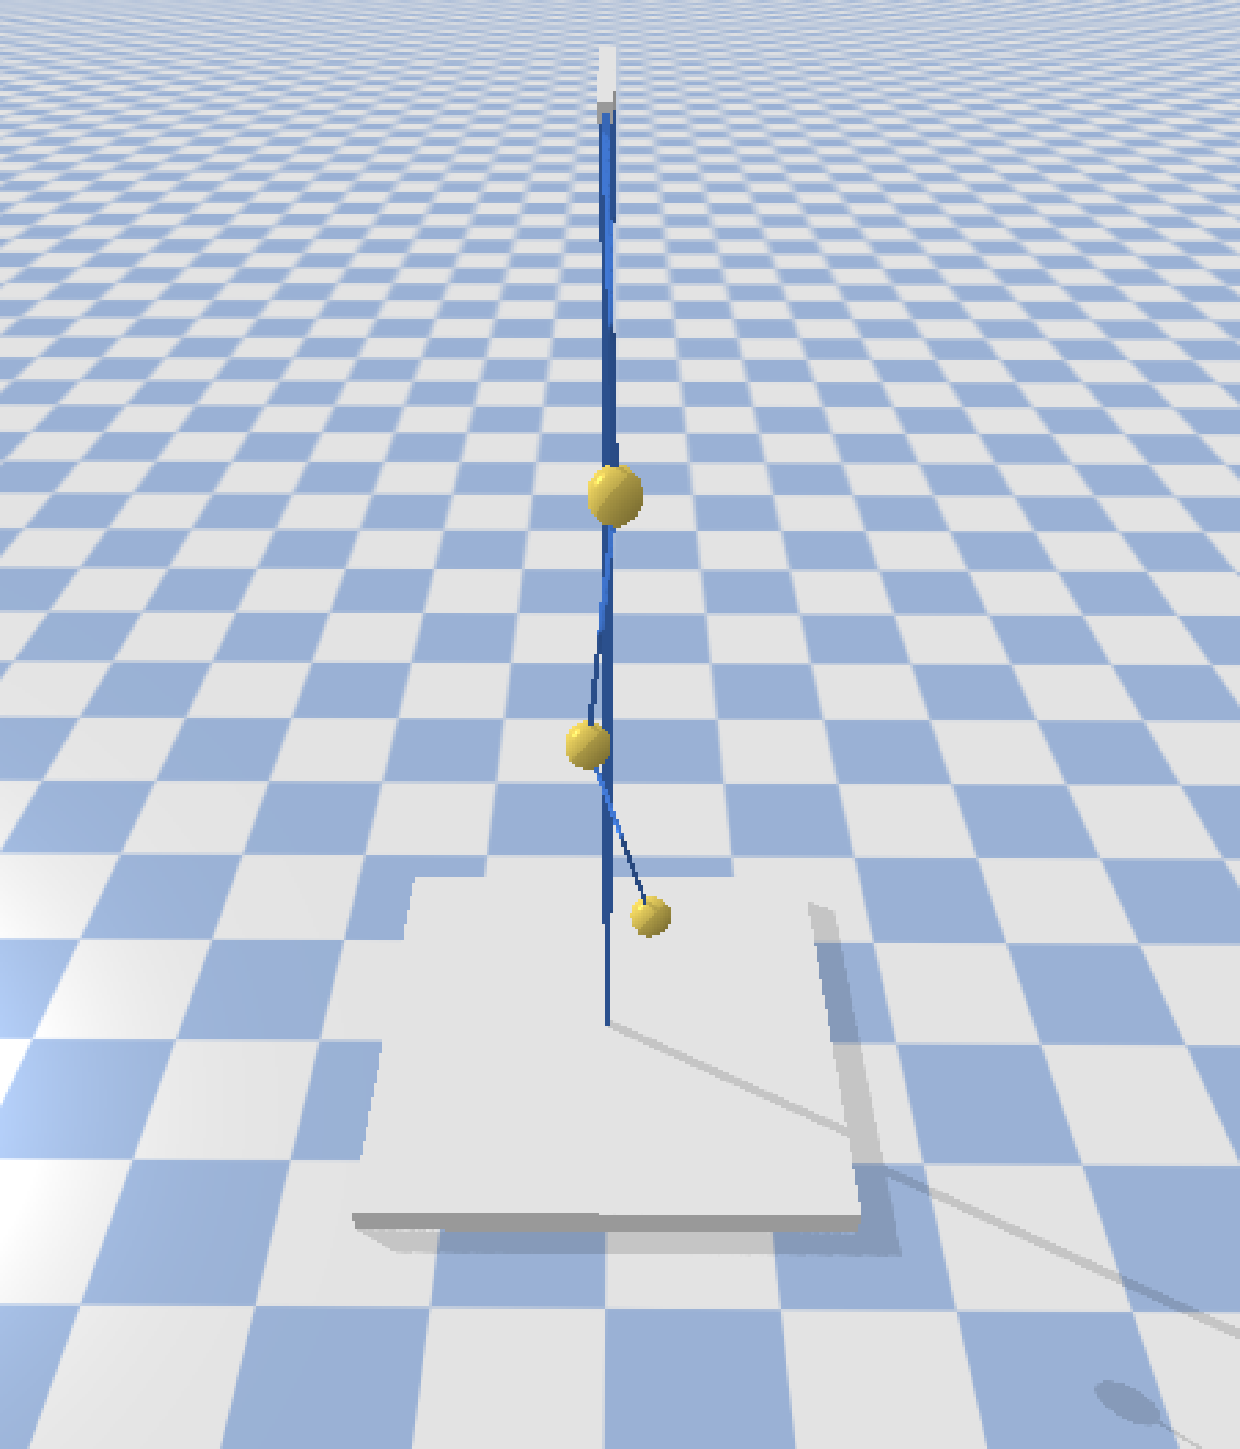
\includegraphics[width=10cm]{chapters/chapter3/pendelum-1.pdf}
 	\caption{Pendelum with 3 degrees of freedom in pybullet}
 	\label{pyb}
 \end{figure}




 
 


 

